\documentclass{article}
% the driver is not listed here, we assume web.cfg
% lists \ExecuteOptions{dvips} or \ExecuteOptions{dvipsone}
% Standard_transparency.joboptions required to distill this file
\usepackage[designiv,usetemplates,nodirectory]{web}
\usepackage[preview]{graphicxsp}


\title{\texorpdfstring{\textsf{GraphicxSP}\\\textsf{Graphicx} versus \textsf{GraphicxSP}}
    {GraphicxSP: Graphicx versus GraphicxSP}}
\author{D. P. Story}
\university{Acro\negthinspace\TeX.Net}
\email{dpstory@acrotex.net}
\subject{Form XObjects and BP, EP and SP operators, transparency}
\keywords{Distiller, Form XObjects, BP, EP, and SP operators,transparency}

\newcommand{\cs}[1]{\texttt{\char`\\#1}}

\embedEPS[hiresbb,transparencyGroup]{AdobeDon}{graphics/AdobeDon}
\embedEPS[transparencyGroup]{ex}{graphics/example}

\parindent0pt
\setlength{\fboxsep}{0pt}

\begin{document}

\maketitle

\section{Introduction}

We make direct visual comparisons between the results obtained from the
\textsf{graphicx} package versus the \textsf{graphicxsp} package. In the sections
that follow, \textsf{graphicx} image always appears \emph{on the left}, and the
\textsf{graphicxsp} image appears \emph{on the right}.

\section{The \texttt{width}/\texttt{height}/\texttt{scale} options}

\begin{center}
\includegraphics[width=1.5in]{graphics/AdobeDon}
\insertEPS[width=1.5in]{AdobeDon}\\[1ex]
\texttt{width=1.5in}
\end{center}

\goodbreak

\begin{center}
\includegraphics[height=1in]{graphics/AdobeDon}
\insertEPS[height=1in]{AdobeDon}\\[1ex]
        \texttt{height=1in}
\end{center}


\begin{center}
\includegraphics[scale=.5]{graphics/AdobeDon}
\insertEPS[,scale=.5]{AdobeDon}\\[1ex]
\texttt{scale=.5}
\end{center}

\medskip
To my eyes, the \textsf{graphicx} images on the left seems blurrier
than the \textsf{graphicxsp} image and don't magnify as well.

\newpage

\section{Comparing \texttt{bb}}

\vspace{1in}

\begin{center}
\includegraphics[width=.5in,bb=30 50 150 100]{graphics/AdobeDon}\qquad\qquad
\insertEPS[width=.5in,bb=30 50 150 100]{AdobeDon}\\[3ex]
        \texttt{bb=30 50 150 100}
\end{center}

\begin{center}
\includegraphics[width=.5in,bb=30 50 150 100,clip]{graphics/AdobeDon}\qquad\qquad
\insertEPS[width=.5in,bb=30 50 150 100,clip]{AdobeDon}\\[1ex]
        \texttt{bb=30 50 150 100,clip}
\end{center}

\newpage

\section{trim}

\begin{center}
\includegraphics[width=.5in,trim=20 20 30 15]{graphics/AdobeDon}\qquad\qquad
\insertEPS[width=.5in,trim=20 20 30 15]{AdobeDon}\\[3ex]
\texttt{trim=20 20 30 15}
\end{center}

\begin{center}

\includegraphics[width=.5in,trim=20 20 30 15,clip]{graphics/AdobeDon}\qquad\qquad
\insertEPS[width=.5in, trim=20 20 30 15,clip]{AdobeDon}\\[1ex]
\texttt{trim=20 20 30 15,clip}
\end{center}

\medskip
Again, to my eyes, the \textsf{graphicx} images on the left seems blurrier
than the \textsf{graphicxsp} image.

\newpage

\section{\protect\texttt{viewport}}

\begin{center}
\includegraphics[width=.5in,viewport=20 20 60 75]{graphics/AdobeDon}\qquad\qquad
\insertEPS[width=.5in, viewport=20 20 60 75]{AdobeDon}\\[4ex]
\texttt{viewport=20 20 60 75}
\end{center}

\begin{center}
\includegraphics[width=.5in,viewport=20 20 60 75,clip]{graphics/AdobeDon}\qquad\qquad
\insertEPS[width=.5in,viewport=20 20 60 75,clip]{AdobeDon}\\[3ex]
\texttt{viewport=20 20 60 75,clip}
\end{center}

\section{\protect\texttt{keepaspectratio}}

\begin{center}
\includegraphics[width=1.5in,height=1in]{graphics/AdobeDon}
\insertEPS[width=1.5in,height=1in]{AdobeDon}\\[1ex]
\texttt{width=1.5in,height=1in}
\end{center}

\begin{center}
\includegraphics[width=1.5in,height=1in,keepaspectratio]{graphics/AdobeDon}
\insertEPS[width=1.5in,height=1in,keepaspectratio]{AdobeDon}\\[1ex]
\texttt{width=1.5in,height=1in,keepaspectratio}
\end{center}

\newpage

\section{rotations}

\begin{center}
\texttt{AdobeDon} \fbox{\includegraphics[width=.5in,origin=c,angle=-45]{graphics/AdobeDon}}
\texttt{AdobeDon} \fbox{\insertEPS[width=.5in,origin=c,angle=-45]{AdobeDon}}\\[1ex]
\texttt{angle=-45,origin=c}
\end{center}

\begin{center}
\texttt{AdobeDon} \fbox{\includegraphics[width=.5in,origin=rt,angle=-45]{graphics/AdobeDon}}
\texttt{AdobeDon} \fbox{\insertEPS[width=.5in,origin=rt,angle=-45]{AdobeDon}}\\[1ex]
\texttt{angle=-45,origin=rt}
\end{center}

\newpage

\section{rotations and \texttt{bb}/\texttt{trim}/\texttt{viewport}}

\begin{center}
\includegraphics[width=.5in,angle=45,bb=30 50 150 100,clip]{graphics/AdobeDon}
\insertEPS[width=.5in,angle=45,bb=30 50 150 100,clip]{AdobeDon}\\[1ex]
\texttt{angle=45,bb=30 50 150 100,clip}
\end{center}

\begin{center}
\includegraphics[width=.5in,angle=45,trim=20 20 30 15,clip]{graphics/AdobeDon}
\insertEPS[width=.5in,angle=45,trim=20 20 30 15,clip]{AdobeDon}\\[1ex]
\texttt{angle=45,trim=20 20 30 15,clip}
\end{center}

\begin{center}
\includegraphics[width=.5in,angle=45,viewport=20 20 60 75,clip]{graphics/AdobeDon}
\insertEPS[width=.5in,angle=45,viewport=20 20 60 75,clip]{AdobeDon}\\[1ex]
\texttt{angle=45,viewport=20 20 60 75,clip}
\end{center}

\newpage

\begin{center}\ifpreview\else\previewtrue\fi
\textbf{MathLab Graphics}\\[1ex]
\insertEPS[width=1in]{ex}
\insertEPS[width=1in,clip]{ex}
\insertEPS[width=1in,transparency={/ca .3}]{ex}\\[1ex]
\textsf{GraphicxSP}: left insert, middle clip, right 30\% transparency
\end{center}

\begin{center}
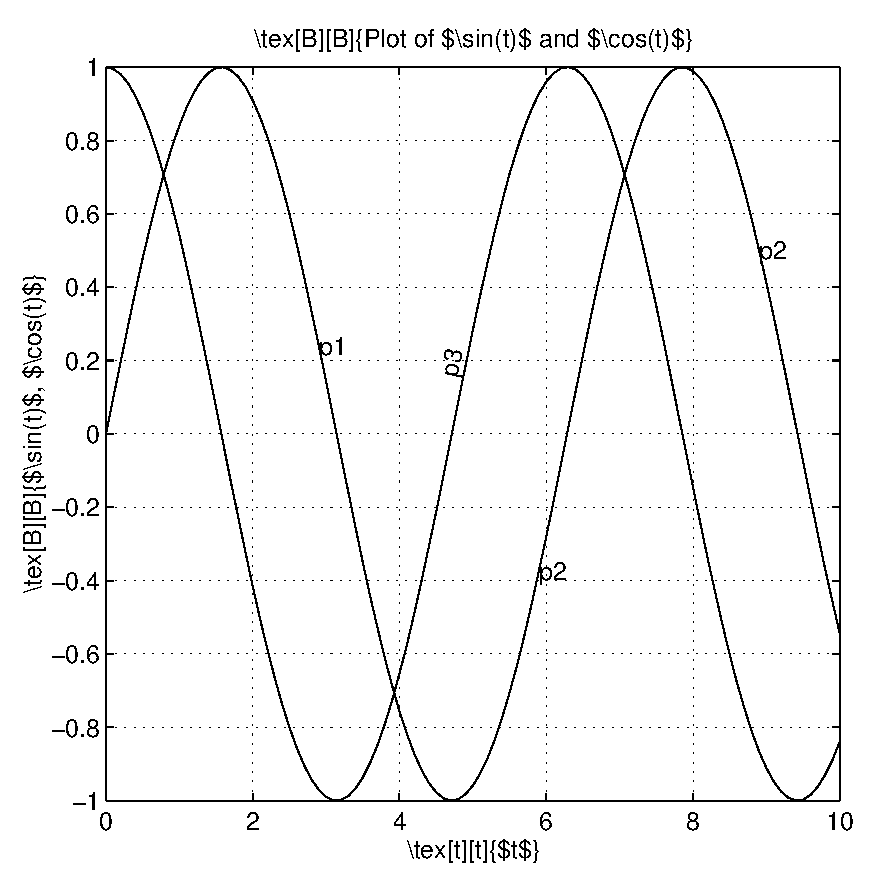
\includegraphics[width=1in]{graphics/example}
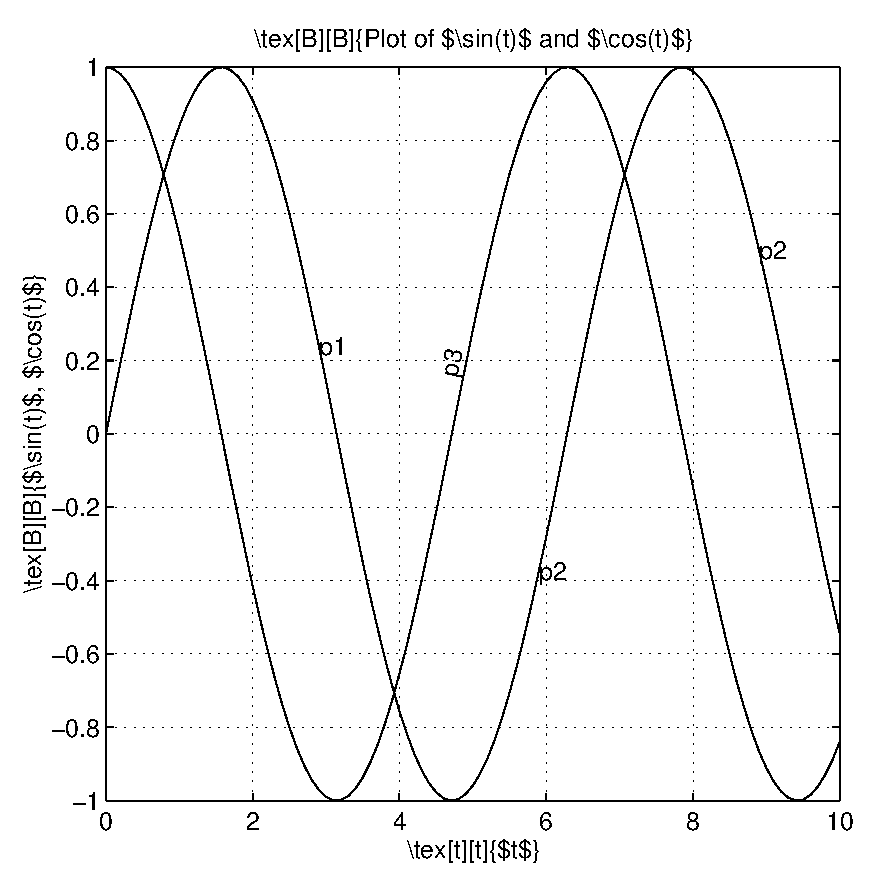
\includegraphics[width=1in,clip]{graphics/example}
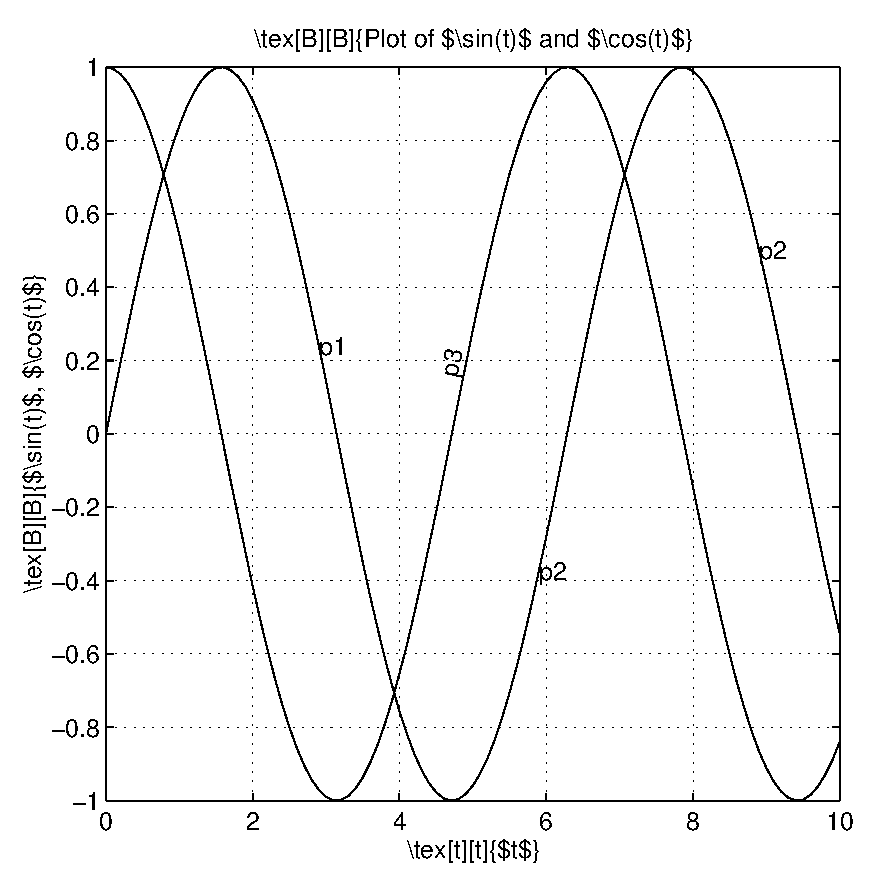
\includegraphics[width=1in]{graphics/example}\\[1ex]
\textsf{Graphicx}: left include, middle clip, right include
\end{center}

The bounding box for this graphic is
\texttt{[\llxOf{ex}\space\llyOf{ex}\space\urxOf{ex}\space\uryOf{ex}]}.


\end{document}

The bounding box for this graphic is
\texttt{[\llxOf{ex}\space\llyOf{ex}\space\urxOf{ex}\space\uryOf{ex}]}.
The figure in the middle has been clipped using its bounding box (the \texttt{clip} option
of \cs{includegraphics/\cs{insertEPS}}), the
one on the right has 30\% opacity and has not been clipped.

\margins{.25in}{.25in}{24pt}{.25in} % left,right,top, bottom
\screensize{5in*\real{0.75}}{5in} % height, width
